\documentclass[11pt, a4paper]{article}

\usepackage{subcaption}

\usepackage{jheppub}
\bibliographystyle{JHEP.bst}
\allowdisplaybreaks

\usepackage{hyperref}
\usepackage{amsmath,amsfonts,amssymb,amsthm,natbib,graphicx,mathtools,mathrsfs}
\usepackage{braket}
\usepackage{enumitem}
\usepackage{slashed}
\usepackage{relsize}
\usepackage{bm}
\usepackage{siunitx}
\usepackage{stackengine}

\newcommand{\ut}[1]{%
  \smash{\ensurestackMath{\stackengine{1pt}{#1}{\scriptscriptstyle\sim}{U}{c}{F}{F}{S}}}
  \vphantom{#1}
}




\makeatletter
\gdef\@fpheader{}
\makeatother

\begin{document}

\title{The Chiral Anomaly in Condensed Matter Systems}
\author{K. Okyere}

\abstract{In this work, the topological nature of Dirac and Weyl semimetals (DSMs and WSMs),
  as well as the chiral anomaly, is outlined using the Berry phase and Atiyah-Singer index theorem.
The use of angle-resolved photoemission spectroscopy in the search for DSMs and WSMs is discussed,
and the most promising materials are identified. Furthermore, the effect of the chiral anomaly
on electron transport in WSMs is deduced, namely, a negative linear magnetoresistance (LMR).
Lastly, the search for the chiral anomaly in WSMs via anomaly-induced negative LMR
is reviewed, and the experimental hurdles introduced by current jetting artefacts
are discussed.}

\maketitle



\section{Introduction}

The concept of quasiparticle dynamics has been an invaluable tool used by
condensed matter physicists to study phenomena in quantum materials
since the creation of Landau's Fermi-liquid theory~\cite{Landau:1956}. Thus, whenever
elementary particle interactions are discovered, condensed matter
physicists are often nearby, searching for their quasiparticle
ramifications in novel quantum materials. This work reviews the search
for Dirac and Weyl semimetals which possess massless Dirac and Weyl fermions
as their quasiparticle excitations~\cite{WSMreview}.
These systems are of great interest in solid-state physics.
In particular, one of the most exotic results in
quantum field theory, the chiral anomaly~\cite{Adler,Bell-Jackiw}, is predicted to manifest in
these materials~\cite{SonSpivak}. We will examine how Dirac and Weyl semimetals are topological
materials, because of their topologically nontrivial electronic band structures,
before outlining the characterisation of the chiral anomaly as a
topological invariant of quantum electrodynamics using the Atiyah-Singer index
theorem~\cite{Atiyah-Singer}. Finally, we will deduce
the effect of the chiral anomaly on magnetoresistance in Weyl semimetals~\cite{SonSpivak}
and review recent efforts to observe this effect.
\section{Background}

\subsection{Relativistic quantum mechanics}
In quantum mechanics, the Schrodinger equation is not Lorentz invariant and is thus
incompatible with special relativity. A generalisation of the relativistic
dispersion relation, using Hamiltonian and momentum operators, leads to the Klein-Gordon
equation~\cite{Klein-tran, Gordon1926}.\footnote{$(\square + \mu^2)\psi = 0; \quad \mu \coloneq \frac{mc}{\hbar}$.}
However, the Klein-Gordon equation is a second-order partial differential equation and
subsequently does not uniquely determine the time-evolution of the wavefunction.
Alternatively, by finding the half-iterate of the d'Alembert
operator,\footnote{$\square \coloneq \frac{1}{c^2}\partial^2_t - \nabla^2$.} the 
Klein-Gordon equation simplifies to a first-order partial differential equation;
the Dirac equation~\cite{dirac1958}
\begin{equation}
  (i\hbar\gamma^\mu\partial_\mu - mc)\psi = 0,
\end{equation}
written using the Einstein summation convention with a
mostly negative metric signature where $\gamma^\mu$
are the Dirac gamma matrices, $m$ is the mass of the Dirac spinor $\psi$,
and $c$ is the speed of light.
The Dirac equation is the Euler-Lagrange equation associated to the Dirac Lagrangian density
\begin{equation}
  \mathcal{L}_D = \bar{\psi}(i\hbar c \gamma^\mu\partial_\mu - mc^2)\psi,
\end{equation}
where the adjoint spinor is defined by
$\bar{\psi} = \psi^\dagger \gamma^0$(cf.~\cite{KofiEthan} for a review on symmetries analytical
mechanics).
This Lagrangian admits a global $\mathrm{U}(1)$ symmetry called the vector symmetry
\begin{equation}
  \psi \mapsto e^{i\vartheta}\psi, \quad \bar{\psi} \mapsto \bar{\psi}e^{-i\vartheta};
  \quad \vartheta \in \mathbb{R}.
\end{equation}
This symmetry corresponds to a conserved current
\begin{equation}
  j^\mu = \bar{\psi}\gamma^\mu\psi,
\end{equation}
called the vector current, via Noether's first theorem~\cite{NoetherTran}.
This vector current is the probability four-current of the Dirac fermion.
Moreover, the vector current is equivalent to the electromagnetic four-current
$J^\mu$;\footnote{$-e j^\mu = J^\mu$}
thus, the conservation of probability is equivalent to the conservation of electric charge
\begin{equation}
  \partial_\mu j^\mu = 0 \iff \partial_t \rho + \bm{\nabla\!\cdot j} = 0,
\end{equation}
where $\rho$ and $\bm{j}$ are the electric charge and current densities respectively.
Using the unitary transformation matrix $U = \frac{1}{\sqrt{2}}(1 + \gamma^5 \gamma^0)$,
the Dirac Lagrangian can be written in the Weyl basis
\begin{equation}
  \gamma^\mu_w = U\gamma^\mu U^\dagger, \quad \psi_w = U \psi,
\end{equation}
\begin{equation}
  \gamma^\mu_w = \begin{pmatrix} 0 & \sigma^\mu \\ \bar{\sigma}^\mu & 0 \end{pmatrix}, \quad 
  \psi_w = \begin{pmatrix} \psi_- \\ \psi_+  \end{pmatrix},
\end{equation}
where $\sigma^\mu$ is the Pauli four-vector, and $\psi_\pm$ are right-handed and left-handed
Weyl spinors respectively~\cite{Weyl-tran}.
Although the Dirac Lagrangian is invariant under this transformation, it is easier to see
in the Weyl basis that when $m=0$ the Dirac Lagrangian admits another $\mathrm{U}(1)$ symmetry
\begin{equation}
  \psi_- \mapsto e^{i\vartheta}\psi_- , \quad
  \psi_+ \mapsto e^{-i\vartheta}\psi_+  \iff
  \psi_w \mapsto e^{i\vartheta\gamma_w^5}\psi_w; \quad \vartheta \in \mathbb{R},
\end{equation}
called the axial symmetry, which has an associated Noether current
\begin{equation}
  j^\mu_5 = \bar{\psi}\gamma^\mu\gamma^5\psi, \quad \partial_\mu j^\mu_5 = 2imc\bar{\psi}\gamma^5\psi,
\end{equation}
known as the axial current.
Furthermore, the massless Dirac equation simplifies to two independent
Weyl equations~\cite{Weyl-tran}
\begin{equation}
  i\hbar\sigma^\mu\partial_\mu \psi_+ = 0, \quad
  i\hbar\bar{\sigma}^\mu\partial_\mu\psi_- =0.
\end{equation}
Chirality is defined by $\gamma^5$; the eigenfunctions of $\gamma^5$
have eigenvalues $\pm 1$,\footnote{n.b. ${(\gamma^5)}^2 = \mathbb{I}_4$.}
and are defined as having positive or negative chirality respectively.
The Weyl spinors $\psi_\pm$ are thus the positive and negative chirality components of
the Dirac spinor.
In the presence of an electromagnetic four-potential $A_\mu$, which we
assume to be a non-dynamical background field so that the Maxwell term of the Lagrangian
for quantum electrodynamics (QED) can be ignored,
the Dirac Lagrangian becomes
\begin{equation}\label{eq:1}
  \mathcal{L} = \bar{\psi}\left( \gamma^\mu \left\{
  i\hbar c \partial_\mu +  e c A_\mu \right\} - mc^2 \right)\psi,
\end{equation}
where $e$ is the elementary charge.\footnote{Here the Dirac spinor has electric charge -$e$.}
In matrix form~\eqref{eq:1} is
\begin{equation}\label{eq:5}
  \mathcal{L} = \psi_w^\dagger
  \begin{pmatrix} c \bar{\sigma}^\mu \widehat{P}_\mu & -mc^2 \\
  -mc^2 & c \sigma^\mu\widehat{P}_\mu  \end{pmatrix}
  \psi_w,
\end{equation}
and in the massless case, the equations of motion are
\begin{equation}
  \sigma^\mu \widehat{P}_\mu \psi_+ = 0, \quad
  \bar{\sigma}^\mu \widehat{P}_\mu \psi_- =0,
\end{equation}
where the four-momentum operator $\widehat{P}_\mu = i\hbar \partial_\mu + e A_\mu$
is given by minimal coupling.
We also notice that
\begin{equation}
  \sigma^\mu \widehat{P}_\mu  = \frac{1}{c}  \left(i \hbar \partial_t + e \phi \right)\mathbb{I}_2
  + \bm{\sigma \cdot} \left( i\hbar \bm{\nabla} + e \bm{A} \right),
\end{equation}
where $\phi$ and $\bm{A}$ are the electric scalar and magnetic vector potentials
respectively, $\bm{\sigma}$ is the Pauli vector, and $\mathbb{I}_2$
is the 2$\times$2 identity matrix. By 
using the definition of four-momentum,\footnote{$P_{\mu} = (\frac{1}{c}E, -\bm{p})$.} we have
the Hamiltonian for Weyl fermions
\begin{equation}\label{eq:2}
  \widehat{H} = - \chi c \bm{\sigma \cdot} (i\hbar \bm{\nabla} + e\bm{A} ) = \chi c
  \bm{\sigma \cdot \hat{p}},
\end{equation}
where $\bm{\hat{p}}$ is the momentum operator, and $\chi =\pm 1$ for right-handed and left-handed
Weyl spinors respectively.

\subsection{Electronic structure and Berry phase}

Insulators are said to be conventional (topologically trivial) if a
continuous transformation (homeomorphism) of lattice parameters can
transform their band structure into the band structure of the vacuum;
the topology is the same as the `atomic limit'. However, not all 
insulators are topologically trivial.
Suppose a system has an initial Hamiltonian, with a discrete non-degenerate 
energy spectrum, that evolves
continuously as $\widehat{H}(\lambda^\mu)$, where $\lambda^\mu(t)$ are $m$
time-dependent parameters.
Furthermore, let $\ket{n(\lambda^\mu(t))}$ be instantaneous eigenstates 
corresponding to energies $E_n(t)$. Assuming that the Hamiltonian evolves slowly 
so that $\braket{m|\partial_t \widehat{H}|n} \approx 0$ (the adiabatic approximation),
then an initial eigenstate evolves as
\begin{equation}
  \ket{n(t = t_0)} \xrightarrow{t \rightarrow t_1} e^{i \theta_n(t_1) +i \phi_n(t_1)}\ket{n(t_0)},
\end{equation}
where $\theta_n(t)$ and $\phi_n(t)$ are the dynamical and Berry phases respectively
\begin{equation}
\theta_n(t_1) = -\frac{1}{\hbar}\int_{t_0}^{t_1}{E_n(\tau)\,d\tau},
\end{equation}
\begin{equation}\label{eq:9}
  \phi_n(t_1) = i\int_{t_0}^{t_1}{\braket{n |\partial_{\mu}| n}
  \frac{d\lambda^\mu}{d\tau} \,d\tau}
  = i\int_C{ \braket{n |\partial_\mu| n}\,d\lambda^\mu };
  \qquad \partial_\mu \coloneq \frac{\partial}{\partial \lambda^\mu},
\end{equation}
where $C$ is a rectifiable curve in $\lambda$-space.
This is the adiabatic theorem~\cite{AdiabaticThrm,Berry},
and \eqref{eq:9} describes how the phase of eigenstates changes as
the system evolves through parameter space.
We now define the Berry potential/connection as
\begin{equation}
  A_\mu^{\bm{\lambda}} =  i \braket{n |\partial_\mu| n}.
\end{equation}
In quantum mechanics, the phase of the eigenstates is unphysical,
the observable quantities are phase differences;
hence, changing the phase of $\ket{n}$ should leave the equations of motion unchanged.
Subsequently, the system is invariant under the transformation
\begin{equation}
  \ket{n} \rightarrow e^{i\beta(\lambda)}\ket{n(\lambda)}
  \implies A_\mu^{\bm{\lambda}} \rightarrow A_\mu^{\bm{\lambda}} - \partial_\mu \beta(\lambda);
  \quad \beta(\lambda^\mu) \in C^2(\mathbb{R}^m),
\end{equation}
This redundancy is similar to gauge freedom in electromagnetism and
leaves the Berry phase invariant if the path through parameter space is a closed path.
Hence, we can construct a $\mathrm{U(1)}$ gauge theory for cyclic variations of
$\widehat{H}(\lambda^\mu)$, analogous to electromagnetism,
where the Berry potential is the gauge connection and the corresponding
field strength
\begin{equation}
  \Omega^{\bm{\lambda}}_{\mu\nu} = \partial_\mu A^{\bm{\lambda}}_\nu -
  \partial_\nu A^{\bm{\lambda}}_\mu,
\end{equation}
is called the Berry curvature. In three dimensions, we also define the Berry curvature
pseudovector
\begin{equation}\label{eq:3}
  \bm{\Omega^\lambda} = \bm{\nabla_{\!\lambda}\!\times} \bm{A^\lambda}.
\end{equation}
Notice that the pseudovector is divergence-free because it is a curl, so the `Berry flux'
is conserved when the Berry potential is non-singular.
Moreover, the antisymmetric tensor and pseudovector are related via
\begin{equation}
  \Omega^{\bm{\lambda}}_{\mu\nu} = \epsilon_{\mu\nu\rho} \Omega^{\bm{\lambda}}_{\rho},
\end{equation}
where $\epsilon_{\mu\nu\rho}$ is the Levi-Civita symbol.
The Berry curvature is a gauge invariant quantity thus, using Stokes' theorem~\cite{StokesThrm},
we can construct another expression for the Berry phase
\begin{equation}
  \phi_n = \oint_C{A^{\bm{\lambda}}_\mu\,d\lambda^\mu} =
  \int_S{\Omega^{\bm{\lambda}}_{\mu\nu}\,ds^\mu\wedge ds^\nu},
\end{equation}
where $C$ is the boundary of the surface $S$ in parameter space. The right-hand side
is the integral of the curvature form of a vector bundle on a
smooth manifold hence by using Chern-Weil theory
we have that
\begin{equation}
  \phi_n = 2\pi c_1,
\end{equation}
where $c_1$ is the first Chern class which is a topologically
invariant integer~\cite{Chern},
also known as the Thouless-Kohmoto-Nightingale-Nijs (TKNN) invariant because of its relation to
the quantum Hall effect~\cite{TKNN}.
Bloch's theorem states that the energy eigenstates of the
$n^\text{th}$ band of a perfect lattice are of the form
\begin{equation}
  \psi_{n\bm{k}}(\bm{r}) = e^{i\bm{k}\cdot\bm{r}}u_{n\bm{k}}(\bm{r}),
\end{equation}
where $\hbar\bm{k}$ is crystal momentum, and the Bloch functions
$u_{n\bm{k}}(\bm{r})$ have the periodicity of the direct lattice~\cite{Bloch}.
Thus, for a crystal lattice the Berry potential becomes 
\begin{equation}
  \bm{A}_{n}^{\bm{k}} =  i\braket{u_{n\bm{k}} |\bm{\nabla_{\! k}}| u_{n\bm{k}}},
\end{equation}
where $n$ is now the band index, and we have that
\begin{equation}\label{eq:11}
  \int{\Omega^{n \bm{k}}_{\mu\nu}\,ds^\mu\wedge ds^\nu} = 2\pi c,
\end{equation}
is a  a topological invariant, where $c$ is called the Chern number.
For 2D crystals~\eqref{eq:11} can be an integral over the Brillouin zone, 
and we have a Chern number associated to each band.
The electronic bands of topologically trivial insulators have a Chern number of 0,
and the most famous Chern insulator (material characterised by Chern numbers)
is the Haldane model of graphene~\cite{Haldane}.
At the interface between topological and conventional insulators the different 
topological invariants force band degeneracy at the boundary and the adiabatic theorem does not
apply. Subsequently, 2D topological insulators have topologically protected metallic 
surface states because the vacuum is topologically trivial.
Thus far, we have seen Chern numbers used to classify two dimensional 
topological insulators but they can also characterise three dimensional materials
; specifically, Dirac and Weyl semimetals.
\section{Dirac and Weyl semimetals}

Weyl semimetals (WSMs) are materials possessing Weyl fermions as their quasiparticle
excitations. Specifically, WSMs are zero band gap semimetals where the effective Hamiltonian
near band degeneracies, called Weyl points, takes the form
\begin{equation}\label{eq:4}
  \widehat{H}(\bm{k}) = \varepsilon_0 \mathbb{I}_2
  + \chi \hbar v_{\! f} \bm{\sigma \cdot} (\bm{k} - \bm{k}^w),
\end{equation}
where $\varepsilon_0$ and $\hbar\bm{k}^w$ are the energy and crystal momentum at the 
Weyl point respectively,\footnote{$\epsilon_0$ is near the Fermi energy.}
$v_{\! f}$ is the Fermi velocity, and $\chi= \pm 1$ is the Weyl point's chirality~\cite{WSMreview}. 
When $\epsilon_0$ is approximately the Fermi energy the quasiparticle excitations
are Weyl fermions because the equations of motion of the WSM Hamiltonian
are the same as~\eqref{eq:2}.
In addition, the von Neumann-Wigner theorem
ensures that Weyl points are isolated in 
the Brillouin zone creating `Weyl cones' at band crossings~\cite{AvoidedCrossing}.
By direct computation, and assuming $\bm{k}^w = 0$ for now,
we find that the eigenstates of the WSM Hamiltonian are 
\begin{equation}
  v_{\pm} = \begin{pmatrix} k_3 \pm |\bm{k}| \\ k_1 +ik_2 \end{pmatrix}; 
  \quad \varepsilon_\pm = \varepsilon_0 \pm \chi \hbar v_{\!f} |\bm{k}|,
\end{equation}
with energies $\varepsilon_\pm$ respectively. Using \eqref{eq:3},
this corresponds to a Berry curvature pseudovector of
\begin{equation}
\boldsymbol{\Omega}^{\bm{k}} = \frac{\chi (\bm{k}-\bm{k}^w)}{2{|\bm{k}-\bm{k}^w|}^3}.
\end{equation}
Thus, using the divergence theorem~\cite{Divthrm} we can see that
Weyl points are monopoles of Berry flux and have Chern number $\chi$
\begin{equation}
  \oint_S{\Omega^{\bm{k}}_{\mu\nu}\,ds^\mu\wedge ds^\nu} = 2\pi\chi,
\end{equation}
where the surface $S$ encloses a Weyl point at $\bm{k}^w$~\cite{SonSpivak}.
Thus, Weyl points are topologically protected band crossings because a homeomorphism
cannot remove them without changing the Chern number (unless two Weyl points are
brought together).
Alternatively, Weyl nodes can be viewed as possessing a `topological charge' $\chi$,
and the Nielsen-Ninomiya theorem, which shows that Weyl
points come in pairs of opposite chirality, represents the conservation
of this topological charge~\cite{Nielsen-Ninomiya}.
Crystals with inversion symmetry\footnote{i.e. $\bm{k}\equiv -\bm{k}$.} have 
symmetric Berry curvatures ($\bm{\Omega^k} = \bm{\Omega}^{-\bm{k}} $).
However, when a crystal has time-reversal symmetry ($\ket{u_{\bm{-k}}} = \ket{u_{\bm{k}}}^\dagger$)
the Berry potential is
\begin{equation}
  A_\mu = \braket{u_{-\bm{k}}^\dagger|\partial_\mu u_{-\bm{k}}^\dagger}
  = \braket{\partial_\mu u_{-\bm{k}}| u_{-\bm{k}}},
\end{equation}
and the Berry curvature is antisymmetric
\begin{equation}
\begin{split}
  \Omega^{\bm{k}}_{\mu\nu} &= \partial_\mu \braket{\partial_\nu u_{-\bm{k}}| u_{-\bm{k}}}
  - \partial_\nu 
  \braket{\partial_\mu u_{-\bm{k}}| u_{-\bm{k}}} \\
        & = \braket{\partial_\nu u_{-\bm{k}}| \partial_\mu u_{-\bm{k}}} -
        \braket{\partial_\mu u_{-\bm{k}}| \partial_\nu u_{-\bm{k}}} = -\Omega^{-\bm{k}}_{\mu\nu}.
\end{split}
\end{equation}
Subsequently, a WSM can have either time-reversal symmetry, in which case Weyl nodes at
opposite points of the Brillouin zone have the same chirality, or inversion symmetry which
produces Weyl points of the same chirality at opposite points.
Moreover, because the total chirality is 0, the number
of Weyl points in a noncentrosymmetric WSM must be a multiple of 4~\cite{WSMreview}.
A WSM is forbidden from having both symmetries due to Kramers' degeneracy,
eigenstates related via time-reversal are degenerate in time-reversal symmetric systems
with half-integer spin~\cite{Kramers}. Hence, when a crystal possess both symmetries we have
that the energy obeys
\begin{equation}
  E_{\uparrow}(\bm{k}) = E_{\downarrow}(-\bm{k}) = E_{\downarrow}(\bm{k}),
\end{equation}
each band is at least doubly degenerate across the Brillouin zone because the
energy is invariant under spin reversal,
which is not true for~\eqref{eq:4}.
In this case, the Hamiltonian with the required degeneracies is
\begin{equation}
  \widehat{H}(\bm{k}) = \varepsilon_0 \mathbb{I}_4 + \hbar v_{\! f}
  \begin{pmatrix} -\bm{\sigma \cdot} (\bm{k}- \bm{k}^d) & 0 \\
  0 & \bm{\sigma \cdot} (\bm{k} - \bm{k}^d)  \end{pmatrix},
\end{equation}
where $\mathbb{I}_4$ is the 4$\times$4 identity matrix, and there is a fourfold
band crossing at energy $\varepsilon_0$ at $\bm{k}^d$ in the
Brillouin zone. This is identical to the Hamiltonian of massless
Dirac fermions~\eqref{eq:5};
hence, it is the Hamiltonian of the Dirac semimetal (DSM)
whose quasiparticle excitations are massless Dirac fermions~\cite{DSM_Na3Bi}.
Subsequently, we call the degeneracy at $\bm{k}^d$ a Dirac point.
Two Weyl points of opposite chirality coincide at $\bm{k}^d$ so the Dirac point 
has no overall Chern number and is not topologically protected~\cite{WSMreview}.
However, when two Weyl points meet they may annihilate each other 
introducing mass terms into the Hamiltonian similar to~\eqref{eq:5}, and
creating a band gap at $\bm{k}^d$. Consequently, DSMs often have additional symmetries
which necessitate a band crossing, creating stable Dirac points.

\subsection{Magnetic WSMs}

The first hypothesised WSMs were centrosymmetric materials with magnetic ordering 
breaking time-reversal symmetries, often called magnetic WSMs. In particular, 
\textit{ab initio} calculations predicted that the pyrochlore iridates A$_{2}$Ir$_{2}$O$_{7}$
(A = yttrium or a lanthanide) possess an all-in/all-out magnetic structure, where all
Ir magnetic moments on a tetrahedron's vertices point either inward or outward, breaking
time-reversal symmetry~\cite{pyrochlore_abin}. Moreover, pyrochlore iridates were hypothesised to 
have multiple electronic phases dependent on the electronic correlation energy $U$, becoming
WSMs with 24 Weyl points at an intermediate $U \sim$~\qty{1.5}{\electronvolt},
and Mott insulators at $U >$~\qty{2}{\electronvolt}.
Experiments have confirmed the existence of magnetic 
order in pyrochlore iridates and their all-in/all-out structure~\cite{pyrochlore_exp}.
However, the WSM phase has yet to be discovered, although some pyrochlore iridates remain promising
WSM candidates. In particular, the large hall conductivity of Nd$_{2}$Ir$_{2}$O$_{7}$ and its low 
magnetisation, due to antiferromagnetic all-in/all-out order,
suggests that the material's spontaneous hall effect has a topological origin~\cite{pyrochlore_Hall}.


\subsection{Noncentrosymmetric WSMs}

Using first principles calculations, TaAs and similar noncentrosymmetric body-centered-tetragonal
crystals were predicted to have 24 Weyl points across their Brillouin zones and topologically protected
surface states called Fermi arcs~\cite{TaAs_abin}.
The prediction of such materials was particularly important because
previous theoretical WSMs were difficult to synthesise magnetic materials. 
The Berry flux through an open surface between two Weyl points of opposite chirality is non-zero;
thus, each 2D plane between Weyl points is a 2D Chern insulator that must
have metallic edge states~\cite{WSMfermiarc}. These gapless edge states on the Fermi surface
of the WSM boundary are called Fermi arcs and
can be observed using angle-resolved photoemission spectroscopy (ARPES).
Moreover, such metallic states must terminate because planes beyond Weyl points are conventional
insulators; the ends of Fermi arcs are projections of Weyl points onto the Fermi surface.
ARPES employs the photoelectric effect to measure crystal momenta, 
using an ultraviolet (UV) laser incident on a sample to produce
photoelectrons which are analysed in a spectrometer~\cite{ARPES_thry}.
Because the electron momentum parallel to the crystal surface is unaffected by the workfunction
(conserved during photoemission) ARPES is a useful probe of crystal momenta
in 2D materials\footnote{n.b. the momentum of a UV photon is negligible}.
If the material workfunction $\phi$
is known, the binding energy 
\begin{equation}
  E_b = \hbar \nu - \phi - E_k,
\end{equation}
may be inferred, where $\nu$ is the laser frequency and $E_k$ is the photoelectron kinetic
energy measured by an electron spectrometer. Using the
crystal momentum parallel to the surface
\begin{equation}
  \hbar k_{||} = \sqrt{2m_e E_k}\sin{\theta},
\end{equation}
where $m_e$ is the electron mass and $\theta$ is the angle between the photoemission direction 
and surface normal,
the Fermi surface ($E_b = 0$) of a 2D material can be mapped.
ARPES experiments have identified the characteristic Fermi arcs of a WSM
in TaAs with \textit{ab initio} band structure predictions closely matching
observation~\cite{TaAs_exp}.


\subsection{Dirac matter}

Band structure calculations predict that Na$_{3}$Bi and Cd$_{3}$As$_{2}$ are DSMs, each possessing a
pair of symmetry protected Dirac points and
Fermi arcs despite no separation between the Weyl points~\cite{Na3Bi_abin,Cd3As2_abin}.
Na$_{3}$Bi forms hexagonal crystals in the $P6_{3}/mmc$ space group with threefold rotational
symmetry which forbids the existence of a band gap; potential Dirac points are protected
by $C_{3}$ symmetry. Hence, the introduction of a uniaxial strain or an external magnetic field
could destroy the Dirac points via removal of $C_3$ symmetry.
Contrastingly, Cd$_{3}$As$_{2}$ exhibits temperature 
dependent polymorphism, possessing a low-temperature ($<$~\qty{750}{\kelvin})
body-centered-tetragonal $I4_{1}/acd$ phase,
an intermediate-temperature (750--\qty{875}{\kelvin}) primitive tetragonal $P4_{2}/nmc$ phase,
and a high-temperature ($>$~\qty{875}{\kelvin}) face-centered-cubic
$Fm\bar{3}m$ phase~\cite{Cd3As2_structure,Cd3As2_polymorphism}.

Initial \textit{ab initio} electronic structure calculations for Cd$_3$As$_{2}$
were preformed erroneously, using the noncentrosymmetric space group $I4_1cd$ as the low-temperature
polymorph, and subsequently predicted a low-temperature WSM phase~\cite{Cd3As2_abin}.
However, the actual low-temperature centrosymmetric $I4_{1}/acd$ phase has fourfold rotational
symmetry, like the intermediate-temperature phase,
which prevents the opening of a band gap at the hypothesised
Dirac points~\cite{Cd3As2_structure2, Cd3As2_structure}.
ARPES measurements of both Na$_{3}$Bi and Cd$_{3}$As$_{2}$ (in the intermediate-temperature
polymorph) monocrystals show linear dispersion at
potential Dirac points consistent with the presence of Dirac cones within the Brillouin 
zone~\cite{Na3Bi_ARPES,Cd3As2_ARPES}.

\section{The chiral anomaly}

The central mathematical object used to investigate quantum field theories (QFTs) in 
the path integral formalism is the partition function~\cite{rivers1988path}
\begin{equation}
  Z[J] = \int{\mathcal{D}\phi\,\exp{\left[ \frac{i}{\hbar} S[\phi] +
  \frac{i}{\hbar} \int{d^4x\, J(x)\phi(x) }\right]} },
\end{equation}
where $S[\phi]$ is the classical action of the dynamical field $\phi(x)$ which is coupled
to a source field $J(x)$. In particular, the partition function
can be used to express expectation values in a QFT
\begin{equation}
  \frac{1}{Z[0]}\int{\mathcal{D}\phi\,F(x)e^{i\frac{S[\phi]}{\hbar}}} = \braket{F(x)}.
\end{equation}
To calculate path integrals we must perform a wick rotation
(imaginary time substitution) so that the classical action is an integral
over Euclidean spacetime,\footnote{Integrals over Minkowski spacetime are
much harder to manipulate.} after which we can transform the time
axis back to $\mathbb{R}$ via analytic continuation.
Anomalies of a QFT are symmetries of the classical action
which are not preserved when the theory is quantised; 
symmetries violated by quantum processes.
In particular, transformations which are symmetries of the classical action
but not symmetries of the partition function are anomalous.
Because of Noether's first theorem
this manifests as the non-conservation of a classically conserved quantity.
Moreover, the Slavnov–Taylor identities~\cite{Slavnov–Taylor} show that, for symmetries linear in the
fields (such as the vector and axial symmetries), a transformation in the path integral `measure'
of the form
\begin{equation}
  \mathcal{D}\phi \mapsto \mathcal{D}\phi \det{[\mathcal{J}]},
\end{equation}
where $\mathcal{J}$ is a singular Jacobian matrix, is necessary and sufficient for a symmetry
to be anomalous;
anomalies are characterised by singular path integral Jacobians for linear symmetries.
For example, the axial symmetry is famously violated by triangle Feynman diagrams,
resulting in the neutral pion's high decay rate known as the
Adler-Bell-Jackiw (ABJ) anomaly~\cite{Adler,Bell-Jackiw}. As we shall see, 
this anomaly (known as the chiral anomaly outside of particle physics) can be 
viewed as a topological invariant of a QFT (specifically QED) via the Atiyah-Singer index
theorem (cf.~\cite{KofiEthan} for a review)~\cite{Atiyah-Singer}.

\subsection{Quantum field theory}
Because Dirac spinors are anticommuting Grassmann variables, the fermionic path integral
is a Berezin integral~\cite{BerezinBook}.
Consequently, to write the path integral for Dirac fermions we must first
decompose the Dirac spinor and its adjoint using an orthonormal basis $\{ \phi_n(x) \}$, of
eigenfunctions of the Dirac operator
$\slashed{D}$,\footnote{Hereafter we use Feynman slash notation
and $i\hbar \widehat{D}_\mu = \widehat{P}_\mu$.}
and the independent Grassmann variables
$\theta_n$ and $\bar{\xi}_m$
\begin{equation}
  \psi = \sum_n{\theta_n\phi_n(x)} = \sum_n{\theta_n\!\braket{x|n}},
\end{equation}
\begin{equation}
  \bar{\psi} = \sum_m{\bar{\xi}_m\phi^{\dagger}_m(x)} = \sum_m{\bar{\xi}_m\!\braket{m|x}}.
  \end{equation}
Subsequently, the path integral `measure' can be seen as a
Berezin integral `measure' under the coordinate transformation
\begin{equation}
  \theta \mapsto \theta_n\braket{x|n},\quad
  \bar{\xi} \mapsto \bar{\xi}_m\braket{m|x},
\end{equation}
\begin{equation}
  \mathcal{D}\psi\mathcal{D}\bar{\psi}
  = {\left[\det{\braket{x|n}}\det{\braket{m|x}}\right]}^{-1}
  \lim_{\substack{N \rightarrow \infty \\
  M \rightarrow \infty}}{\left\{ \prod_n^N{d\theta_n}\prod_m^M{d\bar{\xi}_m} \right\}}
  = \lim_{N \rightarrow \infty}{\prod_n^N{d\theta_n d\bar{\xi}_n}}.
\end{equation}
Under the local vector symmetry the Dirac spinor becomes
\begin{equation}
  \psi' = \sum_n{\theta_n'\phi_n(x)} ;\quad \theta_n' = e^{i\vartheta(x)}\theta_n,
\end{equation}
and similarly for the adjoint spinor. Subsequently, the path integral measure transformation is
\begin{equation}
  \mathcal{D}\psi\mathcal{D}\bar{\psi} \mapsto
  {\left[\det{\left(e^{i\vartheta(x)\mathbb{I}}\right)}
  \det{\left(e^{-i\vartheta(x)\mathbb{I}}\right)} \right]}^{-1}
  \mathcal{D}\psi\mathcal{D}\bar{\psi},
\end{equation}
where $\mathbb{I}$ is the identity matrix.
Clearly the path integral measure is invariant under the vector symmetry;
thus, by the Slavnov–Taylor identities,
the vector symmetry is retained by the quantum theory and electric charge is conserved.
Contrastingly, this is not the case for the axial transformation;
the axial symmetry is anomalous. The following is an
outline of Fujikawa's proof of the existence of the chiral anomaly~\cite{Fujikawa,Fujikawa2}.
Under the local axial symmetry, the Grassmann variables transform as
\begin{equation}
  \theta_n' = \sum_m{C_{nm} \theta_m}, \quad \bar{\xi}_n' = \sum_m{C_{nm} \bar{\xi}_m},
\end{equation}
\begin{equation}
  C_{nm} = \delta_{nm} +i\int{d^4x\, \vartheta(x)\phi_{n}^{\dagger}(x)\gamma^5\phi_m(x)}.
\end{equation}
Using the identities
\begin{equation}
  \ln{(\mathbb{I} + \epsilon A)} = \epsilon A + \mathcal{O}(\epsilon^2),
\end{equation}
\begin{equation}
  \det\left( e^{A}\right) = e^{\mathrm{Tr}(A)},
\end{equation}
one can see that the path integral measure changes by the Jacobian
\begin{equation}\label{eq:10}
  \begin{split}
    \mathcal{J}[\vartheta] & = {(\det{C})}^{-2} = \exp\left[-2 \mathrm{Tr}(\ln{C}) \right] \\
   & = \exp{\left[-2\mathrm{Tr}\left(i
  \int{d^4x\,  \vartheta(x)\phi_{n}^{\dagger}(x)\gamma^5\phi_m(x)} \right) \right]} \\
   & = \exp{\left[ -2i
  \int{d^4x\,\vartheta(x) \sum_n{\phi_{n}^{\dagger}(x)\gamma^5\phi_n(x)}} \right]}.
  \end{split}
\end{equation}
The sum appearing in the Jacobian is clearly divergent (by orthonormality)
and requires the introduction of a regulator, or ultraviolet cut-off, to evaluate
the integral (cf.~Fujikawa's method~\cite{Fujikawa}).
However, we will explore a more elegant topological approach that utilises
topological and analytical indices,
after demonstrating the relationship between the chiral anomaly
and the axial current. Henceforth, we define the axial anomaly,\footnote{In
this work the axial anomaly is a quantity whereas the chiral anomaly is an equation.}
$\mathcal{A}$, using the Jacobian of the path integral measure
\begin{equation}
  \mathcal{J}[\vartheta] = \exp{\left[ - \int{d^4x\,\vartheta(x) \mathcal{A} } \right]}.
\end{equation}
Under the axial transformation in Euclidean spacetime the partition function becomes
\begin{equation}
  Z'[A] = \int{\mathcal{D}\psi'\mathcal{D}\bar{\psi}'\,
  \exp{\left[ \frac{1}{\hbar} \int{d^4x\, -\frac{1}{4\mu_0 c}F_{\mu\nu}F^{\mu\nu} +
  \bar{\psi}'(i\hbar\slashed{D} -mc)\psi'} \right]}},
\end{equation}
where $F_{\mu\nu}$ is the electromagnetic field tensor, and $\mu_0$ is the vacuum permeability.
This is equivalent to a relabeling of the path integration variables so the partition
function must be invariant. Considering the change in the QED Lagrangian
$\mathcal{L}_{\mathrm{QED}}$, we have
\begin{equation}
  Z[A] = \int{\mathcal{D}\psi\mathcal{D}\bar{\psi}\,\mathcal{J}[\vartheta]
    \exp{ \left[\frac{1}{\hbar c} \int{d^4x\, \mathcal{L}_{\mathrm{QED}} +
         c \vartheta(x)(\partial_\mu j^\mu_5 - 2imc\bar{\psi}\gamma^5\psi) }  \right] } }.
\end{equation}
Thus, to first-order in $\vartheta(x)$ we have
\begin{equation}
  Z[A] = \int{\mathcal{D}\psi\mathcal{D}\bar{\psi}\, \left\{1 + \frac{1}{\hbar } \int{d^4x\,
     \vartheta(x)(\partial_\mu j^\mu_5 - 2imc\bar{\psi}\gamma^5\psi -\mathcal{A})} \right\}
   \exp{\left[ \frac{1}{\hbar c} \int{d^4x\, \mathcal{L}_{\mathrm{QED}} } \right]}}.
\end{equation}
Subsequently, by the fundamental lemma of the calculus of variations~\cite{calcvar} we have
the anomalous divergence for the axial current
\begin{equation}
  \partial_\mu j^\mu_5 = 2imc\bar{\psi}\gamma^5\psi + \mathcal{A},
\end{equation}
which we call the chiral anomaly.
The Dirac operator, $\slashed{D}$, is Hermitian in Euclidean space.
If $\phi_n$ is an eigenfunction of $\slashed{D}$, with a non-zero eigenvalue $\lambda_n$,
then $\gamma^5\phi_n$ is also an eigenfunction
\begin{equation}
  \slashed{D}(\gamma^5\phi_n) = -\gamma^5\slashed{D}(\phi_n) = -\lambda_n\gamma^5\phi_n.
\end{equation}
Moreover, Hermiticity of $\slashed{D}$ implies that $\phi_n$ and $\gamma^5\phi_n$
are orthogonal (as they have different eigenvalues) because of the
spectral theorem~\cite{Spectral}.
When the eigenvalue vanishes $\phi_n$ and $\gamma^5\phi_n$
are called zero modes of the Dirac operator. In addition, $\gamma^5$ is 
Hermitian; hence, the spectral theorem implies there exists an orthonormal
basis that diagonalises $\gamma^5$ and spans $\mathrm{Ker}(\slashed{D})$.
Ignoring the infinitesimal parameter $\vartheta(x)$ for now, only the zero modes contribute
to the integral in~\eqref{eq:10} because of orthonormality, and we have that
\begin{equation}
  \int{d^4x\, \sum_n{\phi^\dagger_n\gamma^5\phi_n}}
  = \sum_n{\int{d^4x\,\phi^{0\dagger}_{n+}\phi^0_{n+}}}
  -\sum_n{\int{d^4x\,\phi^{0\dagger}_{n-}\phi^0_{n-}}} = n_+ - n_-,
\end{equation}
\begin{equation}
  \int{d^4x\, \mathcal{A}} = 2i(n_+ - n_-),
\end{equation}
where $n_\pm$ are the number of positive and negative chirality zero modes, $\phi^0_{n\pm}$,
respectively. This is precisely the analytical index of the Dirac operator 
projected onto the positive chirality subspace
\begin{equation}
  \mathrm{index}(\slashed{D}_{+}) = n_+ - n_-, 
\end{equation}
\begin{equation}
  \slashed{D}_\pm \coloneq \slashed{D}P_{\pm} = \slashed{D}\big|_{\{\pm\}},
\end{equation}
where $P_{\pm} = \frac{1}{2}(1 \pm \gamma^5)$ is the chirality
projection operator.
By the Atiyah–Singer index theorem, this index coincides with the Dirac operator's 
topological index on a compact manifold~\cite{Atiyah-Singer}.
This implies that the chiral anomaly is a topological invariant of quantum electrodynamics
and no regularisation procedure can restore the axial symmetry.
On a four dimensional compact manifold $\Omega$, with no boundary and
Riemannian curvature $R$, the topological index is~\cite{AST-Alvarez-Gaume,DiffGeomGauge}
\begin{equation}
  \mathrm{index}(\slashed{D}_+ ) =  \int_{\Omega}{\hat{A}(\Omega)\mathrm{ch}(F)}.
\end{equation}
The integrand, called the index density, only includes 4-form terms and the curvature
form is given by
\begin{equation}
F = \frac{e}{\hbar}\,dA = \frac{e}{2\hbar}F_{\mu\nu}\, dx^\mu \wedge dx^\nu,
\end{equation}
where $dA$ is the exterior derivative of the four-potential.
The characteristic classes
$\mathrm{ch}(F)$ and $\hat{A}(\Omega)$ are the Chern character
of the curvature form, and Dirac genus of the manifold respectively
\begin{equation}
  \mathrm{ch}(F) = \mathrm{Tr}\left(\exp{\left[ \frac{i}{2\pi}F \right]}\right),
\end{equation}
\begin{equation}
  \hat{A}(\Omega) = \sqrt{ \det{\left( \frac{ \frac{i}{4\pi}R }{ \sinh{\frac{i}{4\pi}R} } \right) } }. 
\end{equation}
Now we choose the manifold $S^{4} = \Omega$ so the Riemannian curvature is 
constant and $\hat{A}(\Omega) = 1$. Thus the index becomes
\begin{equation}
  \mathrm{index}(\slashed{D}_+ ) =  \int_{S^4}{\mathrm{ch}(F)}
  = \frac{1}{2!}{\left(\frac{i}{2\pi}\right)}^2 \int_{S^4}{\mathrm{Tr}(F \wedge F)}.
\end{equation}
Assuming the action due to the Maxwell Lagrangian converges
\begin{equation}\label{eq:8}
  \int_{\mathbb{R}^4}{d^4x\, F_{\mu\nu}F^{\mu\nu}} < \infty \iff 
  A_\mu \xrightarrow{|x| \rightarrow \infty} \frac{\hbar}{e}\partial_{\mu}\vartheta;
  \quad \vartheta(x)\in C^2(\mathbb{R}^4),
\end{equation}
we can stereographically project our problem from $S^4$ to $\mathbb{R}^4$.
Hence $\mathrm{ch}(F)$ coincides with the Dirac operator's
index density in Euclidean space if the gauge fields
are asymptotically `flat' ($A_\mu$ is a pure gauge at infinity)~\cite{JackiwRebbi1977,Belavin}.
Using antisymmetry of the wedge product, we identify the
chiral anomaly in Euclidean spacetime as\footnote{The $-i$ factor disappears in Minkowski spacetime.} 
\begin{equation}
  \partial_\mu j^\mu_5 - 2imc\bar{\psi}\gamma^5\psi =
  \mathcal{A}[A_\mu] = \frac{-ie^2}{16\pi^2\hbar^2}
  \epsilon^{\mu\nu\rho\sigma} F_{\mu\nu}F_{\rho\sigma}.
\end{equation}


\subsection{Condensed matter}

Electron transport phenomena in condensed matter systems
are effectively described by the semiclassical model
of electron dynamics~\cite{Ashcroft:102652}. Our goal is to describe the motion of electrons 
between electron-ion scattering events however, we cannot apply an electron's classical 
equations of motion like in the Drude model due to
the uncertainty principle; simultaneously definite position
and momentum are forbidden. Subsequently, we introduce the $n^\text{th}$ band
electron wave packet in a crystal
\begin{equation}
\psi_n(\bm{r}, t) = \int{\frac{d^3\bm{k}}{{(2\pi)}^3}\,
  g(\bm{k}) \psi_{n\bm{k}} e^{-i\omega_n(\bm{k})t} };
\end{equation}
\begin{equation}
  |\bm{k}' - \bm{k}| > \Delta k \implies g(\bm{k}') \approx 0,
\end{equation}
where $\hbar \omega_n(\bm{k})$ is the energy of the Bloch wavefunction $\psi_{n\bm{k}}$,
the weight function $g(\bm{k})$ determines the distribution of the wave packet,
and $\Delta k$ is much smaller than the dimensions of the Brillouin zone.
The mean velocity of a Bloch electron\footnote{n.b. $v_n = \bm{\nabla_k}\omega_n$.}
is also the group velocity of the wave packet. Thus, we can posit that
the wave packet obeys the semiclassical equations of motion
\begin{equation}
  \dot{\ut{\bm{r}}} = \bm{\nabla_{\! k}} \omega_n(\bm{k}), \quad
  \hbar \dot{\ut{\bm{k}}} = - e\bm{E} - e \dot{\ut{\bm{r}}} \bm{ \times B},
\end{equation}
where $\ut{\bm{r}}$ and $\hbar\ut{\bm{k}}$ are
the wave packet position and crystal momentum respectively,
when the spread of the wave packet is much smaller than
the wavelength of external electric and magnetic fields ($\bm{E}$ and $\bm{B}$).
In the presence of a Berry curvature the wave packet velocity
shifts by $- \dot{\ut{\bm{k}}} \bm{\times} \bm{\Omega}^{\bm{k}}$~\cite{BerryCurveTerm}.
However, due to deviations from a perfect lattice caused by the thermal vibrations
of ions, electron-ion scattering occurs in real crystals and the electron distribution function
$f(\ut{\bm{r}}, \ut{\bm{k}}, t)$ does not obey the semiclassical equations of motion. Instead,
we have the Boltzmann kinetic equation
\begin{equation}
\frac{\partial f}{\partial t} + \dot{\ut{\bm{r}}} \bm{ \cdot}
\bm{\nabla}_{\! \scriptsize{\ut{\bm{r}}} }{f}
+ \dot{\ut{\bm{k}}} \bm{\cdot} \bm{\nabla}_{\! \scriptsize{\ut{\bm{k}} }}{f} =
{\left(\frac{\partial f}{\partial t} \right)}_{\!\text{coll}},
\end{equation}
where the collision term on the right-hand side encodes
the effect of scattering on electron transport~\cite{BKE}.
Using the semiclassical phenomenological equations of
motion and the Boltzmann kinetic equation one can derive the hydrodynamic equation~\cite{SonSpivak}
\begin{equation}
  \partial_t N^\pm + \bm{\nabla_{\! r}} \bm{j}^\pm =
  \frac{\chi e^2}{4\pi^2\hbar^2c} \bm{E} \cdot \bm{B},
\end{equation}
where $N^{\pm}$ and $\bm{j}^\pm$ are the electron and current densities at Weyl points
of chirality $\chi =\pm 1$ respectively.
The sums of the chiral specific electron and current densities are the total 
electron and electric current densities respectively ($N$ and $\bm{j}$);
however, their differences ($N^+ - N^-$ and $\bm{j}^+ - \bm{j}^-$) are the
axial charge and 3-current densities respectively
\begin{equation}\label{eq:6}
  \partial_t N + \bm{\nabla_{\! r}} \bm{j} = 0,
\end{equation}
\begin{equation}\label{eq:7}
  \partial_t (N^+ - N^-) + \bm{\nabla_{\! r}} (\bm{j}^+ - \bm{j}^-) =
  \frac{e^2}{2\pi^2\hbar^2c} \bm{E} \cdot \bm{B},
\end{equation}
\eqref{eq:6} represents the conservation of electric charge whereas~\eqref{eq:7}
is the chiral anomaly.\footnote{n.b. $\epsilon^{\mu\nu\rho\sigma} F_{\mu\nu}F_{\rho\sigma.}
= \frac{8}{c} \bm{E \cdot B}$.}
This non-conservation of axial charge is seen as a large electric current between Weyl points of
opposite chirality that conserves the overall electric charge of a Weyl semimetal.
This produces a large negative longitudinal magnetoresistance (LMR)
in WSMs, when external electric and magnetic fields are parallel,
that is highly anisotropic due to the $\bm{E \cdot B}$ factor.


\section{Magnetoresistance experiments}


\begin{figure}[h!]  \centering
  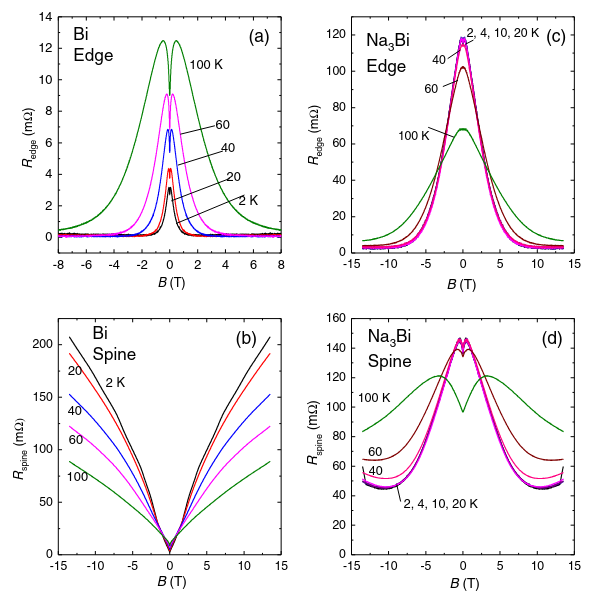
\includegraphics[width=0.7\textwidth]{squeezetest.png}
  \caption{\cite{Squeezetest}Squeeze test results in pure Bi and Na$_3$Bi at various temperatures
  shown on the left and right respectively.}\label{fig:1}
\end{figure}

Current jetting artefacts are of high concern when conducting magnetoresistance experiments in
semimetals with high carrier mobilities. In the presence of a large magnetic field colinear
to the electric current the cyclotronic motion of charge carriers increases the transverse
resistance, but the longitudinal resistance is unchanged~\cite{Squeezetest}.
Subsequently, the electric current
forms a narrow jet in the longitudinal direction between the current contacts on the material,
resulting in a low current density at the edges of a sample.
Thus, the voltage dropped at the edge of the material is lower than the
on-axis potential difference. If the former is detected instead of the latter the reduced voltage 
would be interpreted as an increased longitudinal conductivity; a negative linear magnetoresistance.
This effect is hypothesised to be most pronounced in high-mobility semimetals such as
Bi~\cite{BiMobility,Squeezetest}.

To identify extrinsic negative LMRs caused by current jetting artefacts one
employs the `squeeze test' on semimetal samples,
where pairs of voltage contacts are placed along 
the current contact central axis (along the `spine') and 
along the material edge parallel to the central axis.
These contacts simultaneously measure the spine and edge voltages
($V_\text{spine}$ and $V_\text{edge}$ respectively) from which the effective
resistances are
calculated ($R_\text{spine}(\bm{B})$ and $R_\text{edge}(\bm{B})$ respectively).
The current jetting artefacts produce an increasing $R_\text{edge}(\bm{B})$ and decreasing
$R_\text{spine}(\bm{B})$; consequently, opposite trends in the effective resistances is indicative of
an extrinsic spurious negative LMR~\cite{Squeezetest}.
The opposite trends in the edge and spine effective resistances in Fig.\ref{fig:1} for
pure Bi suggest that the apparent negative magnetoresistance at the Bi edge is
due to current jetting. Contrastingly, the correlation between edge and spine resistances 
within Na$_3$Bi, a low-mobility semimetal, implies an intrinsic negative magnetoresistance.


Magnetoresistance experiments have observed a weak negative LMR in TaAs below
\qty{75}{\kelvin} with high anisotropy~\cite{TaAs}. 
However, due to the high carrier mobility of TaAs
current jetting artefacts arise at $\bm{B} \sim$ \qty{0.4}{\tesla} which is far below
the field strength at which an anomaly induced negative LMR
is expected to manifest ($\bm{B} \sim$ \qty{7}{\tesla})~\cite{Squeezetest}.
Consequently, an anomaly induced negative magnetoresistance is impossible
to identify in TaAs and previously observed LMRs are likely extrinsic.


Contrastingly, evidence for the chiral anomaly is more promising in DSMs.
An external $\bm{B}$ field breaks the time-reversal symmetry of 
the DSM Na$_3$Bi, splitting both Dirac points into
Weyl points of opposite chirality~\cite{DSM_Na3Bi}.
Thus, Na$_3$Bi exhibits an anisotropic negative
magnetoresistance below \qty{100}{\kelvin}~\cite{Squeezetest}.
Moreover, the low carrier mobility of Na$_3$Bi excludes current jetting effects,
suggesting that the negative LMR is intrinsic and
the strongest evidence for the chiral anomaly in condensed matter.

\section{Conclusion}

We have seen how Dirac and Weyl semimetals can be classified as topological
materials and that this gives rise to topologically protected Fermi arcs on their
Fermi surfaces. Similarly, the nature of the chiral anomaly as a topological
invariant of quantum electrodynamics has been laid out. Moreover, 
evidence for existing Dirac and Weyl semimetals has been reviewed, with ARPES
providing strong evidence for the WSM candidate TaAs, and the DSM candidates
Na$_3$Bi and Cd$_3$As$_2$. Using the semiclassical model of electron dynamics
and the Boltzmann kinetic equation, the anomaly-induced negative linear
magnetoresistance in WSMs has been derived. Evidence for the chiral anomaly
in WSMs like TaAs is poor due to their high carrier mobilities producing current jetting
artefacts. The DSM Na$_3$Bi has a low carrier mobility which precludes current
jetting. Hence, the negative linear magnetoresistance observed in Na$_3$Bi is 
the best evidence for the chiral anomaly in condensed matter systems to date.

\vspace*{-5pt}
\bibliography{refs}

\section{Lay summary}

The elementary particles of the universe, which are the building blocks of all matter,
come in mirror-image pairs; electrons can either be left-handed or right-handed.
This handedness property is called chirality, and under normal circumstances,
the number of left-handed and right-handed particles remains constant.
Additionally, electrons obey the conservation of mass; the total number of electrons
is always the same. Some hypothetical fundamental particles, specifically Weyl
fermions, are predicted to violate this conservation law in a process
called the chiral anomaly. In particular, some Weyl fermions are only
left-handed while others are exclusively right-handed.
As a result, the total number of Weyl fermions is not 
necessarily constant; instead, the difference between the number
of left and right-handed Weyl fermions fluctuates according to the chiral anomaly.
Although actual Weyl fermions have not been discovered in nature,
electrons behave as if they were Weyl fermions in materials called Weyl
semimetals. This leads to an imbalance
in the numbers of left and right-handed electrons depending on
the strength of electric and magnetic fields applied to Weyl semimetals.


\end{document}
